\chapter{The Presentation}

When Albert found himself alone with Monte Cristo, “My dear count,”
said he, “allow me to commence my services as \textit{cicerone} by showing you
a specimen of a bachelor’s apartment. You, who are accustomed to the
palaces of Italy, can amuse yourself by calculating in how many square
feet a young man who is not the worst lodged in Paris can live. As we
pass from one room to another, I will open the windows to let you
breathe.”

Monte Cristo had already seen the breakfast-room and the salon on the
ground floor. Albert led him first to his \textit{atelier}, which was, as we
have said, his favorite apartment. Monte Cristo quickly appreciated all
that Albert had collected here—old cabinets, Japanese porcelain,
Oriental stuffs, Venetian glass, arms from all parts of the
world—everything was familiar to him; and at the first glance he
recognized their date, their country, and their origin.

Morcerf had expected he should be the guide; on the contrary, it was he
who, under the count’s guidance, followed a course of archæology,
mineralogy, and natural history.

They descended to the first floor; Albert led his guest into the salon.
The salon was filled with the works of modern artists; there were
landscapes by Dupré, with their long reeds and tall trees, their lowing
oxen and marvellous skies; Delacroix’s Arabian cavaliers, with their
long white burnouses, their shining belts, their damasked arms, their
horses, who tore each other with their teeth while their riders
contended fiercely with their maces; \textit{aquarelles} of Boulanger,
representing Notre Dame de Paris with that vigor that makes the artist
the rival of the poet; there were paintings by Diaz, who makes his
flowers more beautiful than flowers, his suns more brilliant than the
sun; designs by Decamp, as vividly colored as those of Salvator Rosa,
but more poetic; \textit{pastels} by Giraud and Müller, representing children
like angels and women with the features of a virgin; sketches torn from
the album of Dauzats’ “Travels in the East,” that had been made in a
few seconds on the saddle of a camel, or beneath the dome of a
mosque—in a word, all that modern art can give in exchange and as
recompense for the art lost and gone with ages long since past.

Albert expected to have something new this time to show to the
traveller, but, to his great surprise, the latter, without seeking for
the signatures, many of which, indeed, were only initials, named
instantly the author of every picture in such a manner that it was easy
to see that each name was not only known to him, but that each style
associated with it had been appreciated and studied by him. From the
salon they passed into the bedchamber; it was a model of taste and
simple elegance. A single portrait, signed by Léopold Robert, shone in
its carved and gilded frame. This portrait attracted the Count of Monte
Cristo’s attention, for he made three rapid steps in the chamber, and
stopped suddenly before it.

It was the portrait of a young woman of five or six-and-twenty, with a
dark complexion, and light and lustrous eyes, veiled beneath long
lashes. She wore the picturesque costume of the Catalan fisherwomen, a
red and black bodice, and golden pins in her hair. She was looking at
the sea, and her form was outlined on the blue ocean and sky. The light
was so faint in the room that Albert did not perceive the pallor that
spread itself over the count’s visage, or the nervous heaving of his
chest and shoulders. Silence prevailed for an instant, during which
Monte Cristo gazed intently on the picture.

“You have there a most charming mistress, viscount,” said the count in
a perfectly calm tone; “and this costume—a ball costume,
doubtless—becomes her admirably.”

“Ah, monsieur,” returned Albert, “I would never forgive you this
mistake if you had seen another picture beside this. You do not know my
mother; she it is whom you see here. She had her portrait painted thus
six or eight years ago. This costume is a fancy one, it appears, and
the resemblance is so great that I think I still see my mother the same
as she was in 1830. The countess had this portrait painted during the
count’s absence. She doubtless intended giving him an agreeable
surprise; but, strange to say, this portrait seemed to displease my
father, and the value of the picture, which is, as you see, one of the
best works of Léopold Robert, could not overcome his dislike to it. It
is true, between ourselves, that M. de Morcerf is one of the most
assiduous peers at the Luxembourg, a general renowned for theory, but a
most mediocre amateur of art. It is different with my mother, who
paints exceedingly well, and who, unwilling to part with so valuable a
picture, gave it to me to put here, where it would be less likely to
displease M. de Morcerf, whose portrait, by Gros, I will also show you.
Excuse my talking of family matters, but as I shall have the honor of
introducing you to the count, I tell you this to prevent you making any
allusions to this picture. The picture seems to have a malign
influence, for my mother rarely comes here without looking at it, and
still more rarely does she look at it without weeping. This
disagreement is the only one that has ever taken place between the
count and countess, who are still as much united, although married more
than twenty years, as on the first day of their wedding.”

\begin{figure}[h]
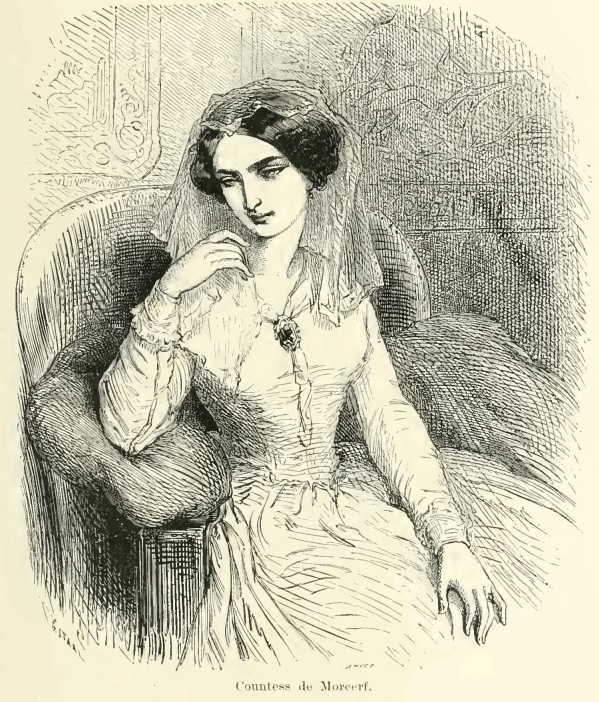
\includegraphics[width=\textwidth]{20261m.jpg}
\end{figure}

Monte Cristo glanced rapidly at Albert, as if to seek a hidden meaning
in his words, but it was evident the young man uttered them in the
simplicity of his heart.

“Now,” said Albert, “that you have seen all my treasures, allow me to
offer them to you, unworthy as they are. Consider yourself as in your
own house, and to put yourself still more at your ease, pray accompany
me to the apartments of M. de Morcerf, he whom I wrote from Rome an
account of the services you rendered me, and to whom I announced your
promised visit, and I may say that both the count and countess
anxiously desire to thank you in person. You are somewhat \textit{blasé} I
know, and family scenes have not much effect on Sinbad the Sailor, who
has seen so many others. However, accept what I propose to you as an
initiation into Parisian life—a life of politeness, visiting, and
introductions.”

Monte Cristo bowed without making any answer; he accepted the offer
without enthusiasm and without regret, as one of those conventions of
society which every gentleman looks upon as a duty. Albert summoned his
servant, and ordered him to acquaint M. and Madame de Morcerf of the
arrival of the Count of Monte Cristo. Albert followed him with the
count. When they arrived at the antechamber, above the door was visible
a shield, which, by its rich ornaments and its harmony with the rest of
the furniture, indicated the importance the owner attached to this
blazon. Monte Cristo stopped and examined it attentively.

“Azure seven merlets, or, placed bender,” said he. “These are,
doubtless, your family arms? Except the knowledge of blazons, that
enables me to decipher them, I am very ignorant of heraldry—I, a count
of a fresh creation, fabricated in Tuscany by the aid of a commandery
of St. Stephen, and who would not have taken the trouble had I not been
told that when you travel much it is necessary. Besides, you must have
something on the panels of your carriage, to escape being searched by
the custom-house officers. Excuse my putting such a question to you.”

“It is not indiscreet,” returned Morcerf, with the simplicity of
conviction. “You have guessed rightly. These are our arms, that is,
those of my father, but they are, as you see, joined to another shield,
which has gules, a silver tower, which are my mother’s. By her side I
am Spanish, but the family of Morcerf is French, and, I have heard, one
of the oldest of the south of France.”

“Yes,” replied Monte Cristo “these blazons prove that. Almost all the
armed pilgrims that went to the Holy Land took for their arms either a
cross, in honor of their mission, or birds of passage, in sign of the
long voyage they were about to undertake, and which they hoped to
accomplish on the wings of faith. One of your ancestors had joined the
Crusades, and supposing it to be only that of St. Louis, that makes you
mount to the thirteenth century, which is tolerably ancient.”

“It is possible,” said Morcerf; “my father has in his study a
genealogical tree which will tell you all that, and on which I made
commentaries that would have greatly edified d’Hozier and Jaucourt. At
present I no longer think of it, and yet I must tell you that we are
beginning to occupy ourselves greatly with these things under our
popular government.”

“Well, then, your government would do well to choose from the past
something better than the things that I have noticed on your monuments,
and which have no heraldic meaning whatever. As for you, viscount,”
continued Monte Cristo to Morcerf, “you are more fortunate than the
government, for your arms are really beautiful, and speak to the
imagination. Yes, you are at once from Provence and Spain; that
explains, if the portrait you showed me be like, the dark hue I so much
admired on the visage of the noble Catalan.”

It would have required the penetration of Œdipus or the Sphinx to have
divined the irony the count concealed beneath these words, apparently
uttered with the greatest politeness. Morcerf thanked him with a smile,
and pushed open the door above which were his arms, and which, as we
have said, opened into the salon. In the most conspicuous part of the
salon was another portrait. It was that of a man, from five to
eight-and-thirty, in the uniform of a general officer, wearing the
double epaulet of heavy bullion, that indicates superior rank, the
ribbon of the Legion of Honor around his neck, which showed he was a
commander, and on the right breast, the star of a grand officer of the
order of the Saviour, and on the left that of the grand cross of
Charles III., which proved that the person represented by the picture
had served in the wars of Greece and Spain, or, what was just the same
thing as regarded decorations, had fulfilled some diplomatic mission in
the two countries.

Monte Cristo was engaged in examining this portrait with no less care
than he had bestowed upon the other, when another door opened, and he
found himself opposite to the Count of Morcerf in person.

He was a man of forty to forty-five years, but he seemed at least
fifty, and his black moustache and eyebrows contrasted strangely with
his almost white hair, which was cut short, in the military fashion. He
was dressed in plain clothes, and wore at his button-hole the ribbons
of the different orders to which he belonged.

He entered with a tolerably dignified step, and some little haste.
Monte Cristo saw him advance towards him without making a single step.
It seemed as if his feet were rooted to the ground, and his eyes on the
Count of Morcerf.

“Father,” said the young man, “I have the honor of presenting to you
the Count of Monte Cristo, the generous friend whom I had the good
fortune to meet in the critical situation of which I have told you.”

“You are most welcome, monsieur,” said the Count of Morcerf, saluting
Monte Cristo with a smile, “and monsieur has rendered our house, in
preserving its only heir, a service which insures him our eternal
gratitude.”

As he said these words, the count of Morcerf pointed to a chair, while
he seated himself in another opposite the window.

Monte Cristo, in taking the seat Morcerf offered him, placed himself in
such a manner as to remain concealed in the shadow of the large velvet
curtains, and read on the careworn and livid features of the count a
whole history of secret griefs written in each wrinkle time had planted
there.

“The countess,” said Morcerf, “was at her toilet when she was informed
of the visit she was about to receive. She will, however, be in the
salon in ten minutes.”

“It is a great honor to me,” returned Monte Cristo, “to be thus, on the
first day of my arrival in Paris, brought in contact with a man whose
merit equals his reputation, and to whom fortune has for once been
equitable, but has she not still on the plains of Mitidja, or in the
mountains of Atlas, a marshal’s staff to offer you?”

“Oh,” replied Morcerf, reddening slightly, “I have left the service,
monsieur. Made a peer at the Restoration, I served through the first
campaign under the orders of Marshal Bourmont. I could, therefore,
expect a higher rank, and who knows what might have happened had the
elder branch remained on the throne? But the Revolution of July was, it
seems, sufficiently glorious to allow itself to be ungrateful, and it
was so for all services that did not date from the imperial period. I
tendered my resignation, for when you have gained your epaulets on the
battle-field, you do not know how to manœuvre on the slippery grounds
of the salons. I have hung up my sword, and cast myself into politics.
I have devoted myself to industry; I study the useful arts. During the
twenty years I served, I often wished to do so, but I had not the
time.”

“These are the ideas that render your nation superior to any other,”
returned Monte Cristo. “A gentleman of high birth, possessor of an
ample fortune, you have consented to gain your promotion as an obscure
soldier, step by step—this is uncommon; then become general, peer of
France, commander of the Legion of Honor, you consent to again commence
a second apprenticeship, without any other hope or any other desire
than that of one day becoming useful to your fellow-creatures; this,
indeed, is praiseworthy,—nay, more, it is sublime.”

\begin{figure}[ht]
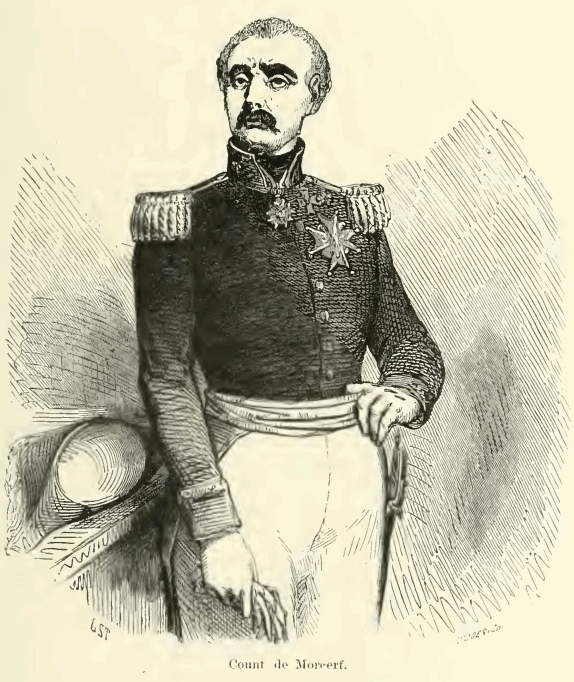
\includegraphics[width=\textwidth]{20265m.jpg}
\end{figure}

Albert looked on and listened with astonishment; he was not used to see
Monte Cristo give vent to such bursts of enthusiasm.

“Alas,” continued the stranger, doubtless to dispel the slight cloud
that covered Morcerf’s brow, “we do not act thus in Italy; we grow
according to our race and our species, and we pursue the same lines,
and often the same uselessness, all our lives.”

“But, monsieur,” said the Count of Morcerf, “for a man of your merit,
Italy is not a country, and France opens her arms to receive you;
respond to her call. France will not, perhaps, be always ungrateful.
She treats her children ill, but she always welcomes strangers.”

“Ah, father,” said Albert with a smile, “it is evident you do not know
the Count of Monte Cristo; he despises all honors, and contents himself
with those written on his passport.”

“That is the most just remark,” replied the stranger, “I ever heard
made concerning myself.”

“You have been free to choose your career,” observed the Count of
Morcerf, with a sigh; “and you have chosen the path strewed with
flowers.”

“Precisely, monsieur,” replied Monte Cristo with one of those smiles
that a painter could never represent or a physiologist analyze.

“If I did not fear to fatigue you,” said the general, evidently charmed
with the count’s manners, “I would have taken you to the Chamber; there
is a debate very curious to those who are strangers to our modern
senators.”

“I shall be most grateful, monsieur, if you will, at some future time,
renew your offer, but I have been flattered with the hope of being
introduced to the countess, and I will therefore wait.”

“Ah, here is my mother,” cried the viscount.

Monte Cristo, turned round hastily, and saw Madame de Morcerf at the
entrance of the salon, at the door opposite to that by which her
husband had entered, pale and motionless; when Monte Cristo turned
round, she let fall her arm, which for some unknown reason had been
resting on the gilded door-post. She had been there some moments, and
had heard the last words of the visitor. The latter rose and bowed to
the countess, who inclined herself without speaking.

“Ah! good heavens, madame,” said the count, “are you ill, or is it the
heat of the room that affects you?”

“Are you ill, mother?” cried the viscount, springing towards her.

She thanked them both with a smile.

“No,” returned she, “but I feel some emotion on seeing, for the first
time, the man without whose intervention we should have been in tears
and desolation. Monsieur,” continued the countess, advancing with the
majesty of a queen, “I owe to you the life of my son, and for this I
bless you. Now, I thank you for the pleasure you give me in thus
affording me the opportunity of thanking you as I have blessed you,
from the bottom of my heart.”

The count bowed again, but lower than before; he was even paler than
Mercédès.

“Madame,” said he, “the count and yourself recompense too generously a
simple action. To save a man, to spare a father’s feelings, or a
mother’s sensibility, is not to do a good action, but a simple deed of
humanity.”

At these words, uttered with the most exquisite sweetness and
politeness, Madame de Morcerf replied:

“It is very fortunate for my son, monsieur, that he found such a
friend, and I thank God that things are thus.”

And Mercédès raised her fine eyes to heaven with so fervent an
expression of gratitude, that the count fancied he saw tears in them.
M. de Morcerf approached her.

“Madame,” said he. “I have already made my excuses to the count for
quitting him, and I pray you to do so also. The sitting commences at
two; it is now three, and I am to speak.”

“Go, then, and monsieur and I will strive our best to forget your
absence,” replied the countess, with the same tone of deep feeling.
“Monsieur,” continued she, turning to Monte Cristo, “will you do us the
honor of passing the rest of the day with us?”

“Believe me, madame, I feel most grateful for your kindness, but I got
out of my travelling carriage at your door this morning, and I am
ignorant how I am installed in Paris, which I scarcely know; this is
but a trifling inquietude, I know, but one that may be appreciated.”

“We shall have the pleasure another time,” said the countess; “you
promise that?”

Monte Cristo inclined himself without answering, but the gesture might
pass for assent.

“I will not detain you, monsieur,” continued the countess; “I would not
have our gratitude become indiscreet or importunate.”

“My dear Count,” said Albert, “I will endeavor to return your
politeness at Rome, and place my coupé at your disposal until your own
be ready.”

“A thousand thanks for your kindness, viscount,” returned the Count of
Monte Cristo “but I suppose that M. Bertuccio has suitably employed the
four hours and a half I have given him, and that I shall find a
carriage of some sort ready at the door.”

Albert was used to the count’s manner of proceeding; he knew that, like
Nero, he was in search of the impossible, and nothing astonished him,
but wishing to judge with his own eyes how far the count’s orders had
been executed, he accompanied him to the door of the house. Monte
Cristo was not deceived. As soon as he appeared in the Count of
Morcerf’s antechamber, a footman, the same who at Rome had brought the
count’s card to the two young men, and announced his visit, sprang into
the vestibule, and when he arrived at the door the illustrious
traveller found his carriage awaiting him. It was a \textit{coupé} of Koller’s
building, and with horses and harness for which Drake had, to the
knowledge of all the lions of Paris, refused on the previous day seven
hundred guineas.

“Monsieur,” said the count to Albert, “I do not ask you to accompany me
to my house, as I can only show you a habitation fitted up in a hurry,
and I have, as you know, a reputation to keep up as regards not being
taken by surprise. Give me, therefore, one more day before I invite
you; I shall then be certain not to fail in my hospitality.”

“If you ask me for a day, count, I know what to anticipate; it will not
be a house I shall see, but a palace. You have decidedly some genius at
your control.”

“\textit{Ma foi}, spread that idea,” replied the Count of Monte Cristo,
putting his foot on the velvet-lined steps of his splendid carriage,
“and that will be worth something to me among the ladies.”

As he spoke, he sprang into the vehicle, the door was closed, but not
so rapidly that Monte Cristo failed to perceive the almost
imperceptible movement which stirred the curtains of the apartment in
which he had left Madame de Morcerf.

When Albert returned to his mother, he found her in the boudoir
reclining in a large velvet armchair, the whole room so obscure that
only the shining spangle, fastened here and there to the drapery, and
the angles of the gilded frames of the pictures, showed with some
degree of brightness in the gloom. Albert could not see the face of the
countess, as it was covered with a thin veil she had put on her head,
and which fell over her features in misty folds, but it seemed to him
as though her voice had altered. He could distinguish amid the perfumes
of the roses and heliotropes in the flower-stands, the sharp and
fragrant odor of volatile salts, and he noticed in one of the chased
cups on the mantle-piece the countess’s smelling-bottle, taken from its
shagreen case, and exclaimed in a tone of uneasiness, as he entered:

“My dear mother, have you been ill during my absence?”

“No, no, Albert, but you know these roses, tuberoses, and
orange-flowers throw out at first, before one is used to them, such
violent perfumes.”

“Then, my dear mother,” said Albert, putting his hand to the bell,
“they must be taken into the antechamber. You are really ill, and just
now were so pale as you came into the room——”

“Was I pale, Albert?”

“Yes; a pallor that suits you admirably, mother, but which did not the
less alarm my father and myself.”

“Did your father speak of it?” inquired Mercédès eagerly.

“No, madame; but do you not remember that he spoke of the fact to you?”

\begin{figure}[ht]
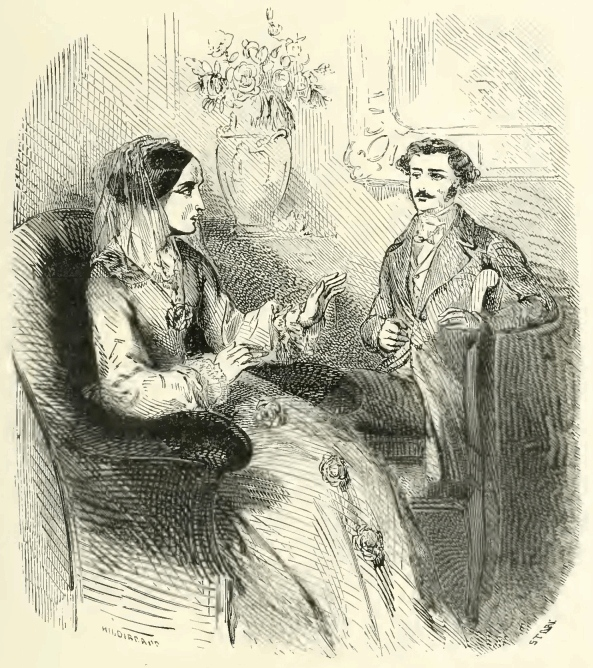
\includegraphics[width=\textwidth]{20269m.jpg}
\end{figure}

“Yes, I do remember,” replied the countess.

A servant entered, summoned by Albert’s ring of the bell.

“Take these flowers into the anteroom or dressing-room,” said the
viscount; “they make the countess ill.”

The footman obeyed his orders. A long pause ensued, which lasted until
all the flowers were removed.

“What is this name of Monte Cristo?” inquired the countess, when the
servant had taken away the last vase of flowers, “is it a family name,
or the name of the estate, or a simple title?”

“I believe, mother, it is merely a title. The count purchased an island
in the Tuscan archipelago, and, as he told you today, has founded a
commandery. You know the same thing was done for Saint Stephen of
Florence, Saint George Constantinian of Parma, and even for the Order
of Malta. Except this, he has no pretension to nobility, and calls
himself a chance count, although the general opinion at Rome is that
the count is a man of very high distinction.”

“His manners are admirable,” said the countess, “at least, as far as I
could judge in the few minutes he remained here.”

“They are perfect mother, so perfect, that they surpass by far all I
have known in the leading aristocracy of the three proudest nobilities
of Europe—the English, the Spanish, and the German.”

The countess paused a moment; then, after a slight hesitation, she
resumed.

“You have seen, my dear Albert—I ask the question as a mother—you have
seen M. de Monte Cristo in his house, you are quicksighted, have much
knowledge of the world, more tact than is usual at your age, do you
think the count is really what he appears to be?”

“What does he appear to be?”

“Why, you have just said,—a man of high distinction.”

“I told you, my dear mother, he was esteemed such.”

“But what is your own opinion, Albert?”

“I must tell you that I have not come to any decided opinion respecting
him, but I think him a Maltese.”

“I do not ask you of his origin but what he is.”

“Ah! what he is; that is quite another thing. I have seen so many
remarkable things in him, that if you would have me really say what I
think, I shall reply that I really do look upon him as one of Byron’s
heroes, whom misery has marked with a fatal brand; some Manfred, some
Lara, some Werner, one of those wrecks, as it were, of some ancient
family, who, disinherited of their patrimony, have achieved one by the
force of their adventurous genius, which has placed them above the laws
of society.”

“You say——”

“I say that Monte Cristo is an island in the midst of the
Mediterranean, without inhabitants or garrison, the resort of smugglers
of all nations, and pirates of every flag. Who knows whether or not
these industrious worthies do not pay to their feudal lord some dues
for his protection?”

“That is possible,” said the countess, reflecting.

“Never mind,” continued the young man, “smuggler or not, you must
agree, mother dear, as you have seen him, that the Count of Monte
Cristo is a remarkable man, who will have the greatest success in the
salons of Paris. Why, this very morning, in my rooms, he made his
\textit{entrée} amongst us by striking every man of us with amazement, not
even excepting Château-Renaud.”

“And what do you suppose is the count’s age?” inquired Mercédès,
evidently attaching great importance to this question.

“Thirty-five or thirty-six, mother.”

“So young,—it is impossible,” said Mercédès, replying at the same time
to what Albert said as well as to her own private reflection.

“It is the truth, however. Three or four times he has said to me, and
certainly without the slightest premeditation, ‘at such a period I was
five years old, at another ten years old, at another twelve,’ and I,
induced by curiosity, which kept me alive to these details, have
compared the dates, and never found him inaccurate. The age of this
singular man, who is of no age, is then, I am certain, thirty-five.
Besides, mother, remark how vivid his eye, how raven-black his hair,
and his brow, though so pale, is free from wrinkles,—he is not only
vigorous, but also young.”

The countess bent her head, as if beneath a heavy wave of bitter
thoughts.

“And has this man displayed a friendship for you, Albert?” she asked
with a nervous shudder.

“I am inclined to think so.”

“And—do—you—like—him?”

“Why, he pleases me in spite of Franz d’Épinay, who tries to convince
me that he is a being returned from the other world.”

The countess shuddered.

“Albert,” she said, in a voice which was altered by emotion, “I have
always put you on your guard against new acquaintances. Now you are a
man, and are able to give me advice; yet I repeat to you, Albert, be
prudent.”

“Why, my dear mother, it is necessary, in order to make your advice
turn to account, that I should know beforehand what I have to distrust.
The count never plays, he only drinks pure water tinged with a little
sherry, and is so rich that he cannot, without intending to laugh at
me, try to borrow money. What, then, have I to fear from him?”

“You are right,” said the countess, “and my fears are weakness,
especially when directed against a man who has saved your life. How did
your father receive him, Albert? It is necessary that we should be more
than complaisant to the count. M. de Morcerf is sometimes occupied, his
business makes him reflective, and he might, without intending it——”

“Nothing could be in better taste than my father’s demeanor, madame,”
said Albert; “nay, more, he seemed greatly flattered at two or three
compliments which the count very skilfully and agreeably paid him with
as much ease as if he had known him these thirty years. Each of these
little tickling arrows must have pleased my father,” added Albert with
a laugh. “And thus they parted the best possible friends, and M. de
Morcerf even wished to take him to the Chamber to hear the speakers.”

The countess made no reply. She fell into so deep a reverie that her
eyes gradually closed. The young man, standing up before her, gazed
upon her with that filial affection which is so tender and endearing
with children whose mothers are still young and handsome. Then, after
seeing her eyes closed, and hearing her breathe gently, he believed she
had dropped asleep, and left the apartment on tiptoe, closing the door
after him with the utmost precaution.

“This devil of a fellow,” he muttered, shaking his head; “I said at the
time he would create a sensation here, and I measure his effect by an
infallible thermometer. My mother has noticed him, and he must
therefore, perforce, be remarkable.”

He went down to the stables, not without some slight annoyance, when he
remembered that the Count of Monte Cristo had laid his hands on a
“turnout” which sent his bays down to second place in the opinion of
connoisseurs.

“Most decidedly,” said he, “men are not equal, and I must beg my father
to develop this theorem in the Chamber of Peers.”
